\subsubsection*{Resultados obtenidos}
%Nota: Al ser los resultados de los experimentos sobre ambos tests muy similares, decidimos analizarlos en conjunto.

\subsubsection*{Tests KNN}

Uno de los aspectos más importantes nuestra experimentación es determinar la cantidad óptima de vecínos cercanos, por eso es que vamos a llevar acabo tests de K con KNN en función de nuestras métricas. Para evitar tener más variables que puedan interferír en nuestra experimencación no utilizamos PCA.


\begin{figure}[H]
\begin{subfigure}[h]{0.62\linewidth}
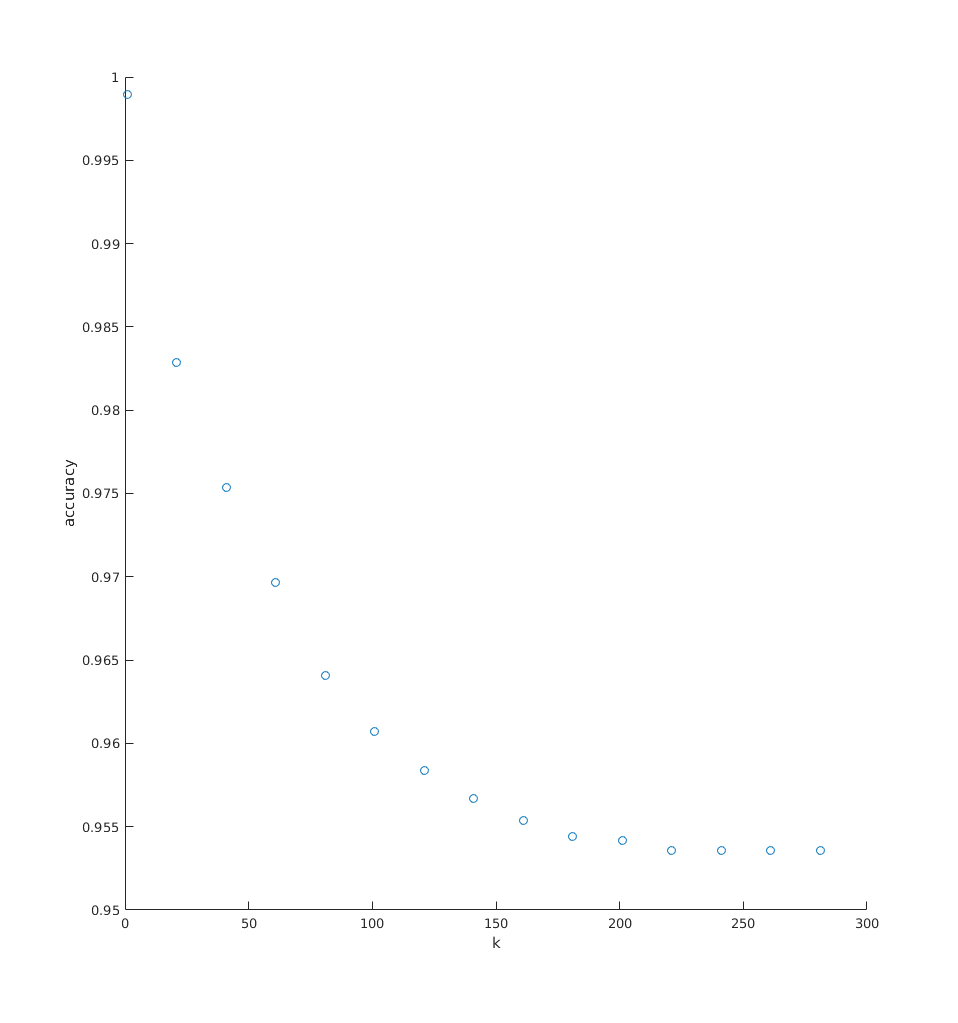
\includegraphics[width=\linewidth]{img/k_knn_accu.png}
\caption{Utilizando imágenes reducidas}
\end{subfigure}
\hfill
\begin{subfigure}[h]{0.62\linewidth}
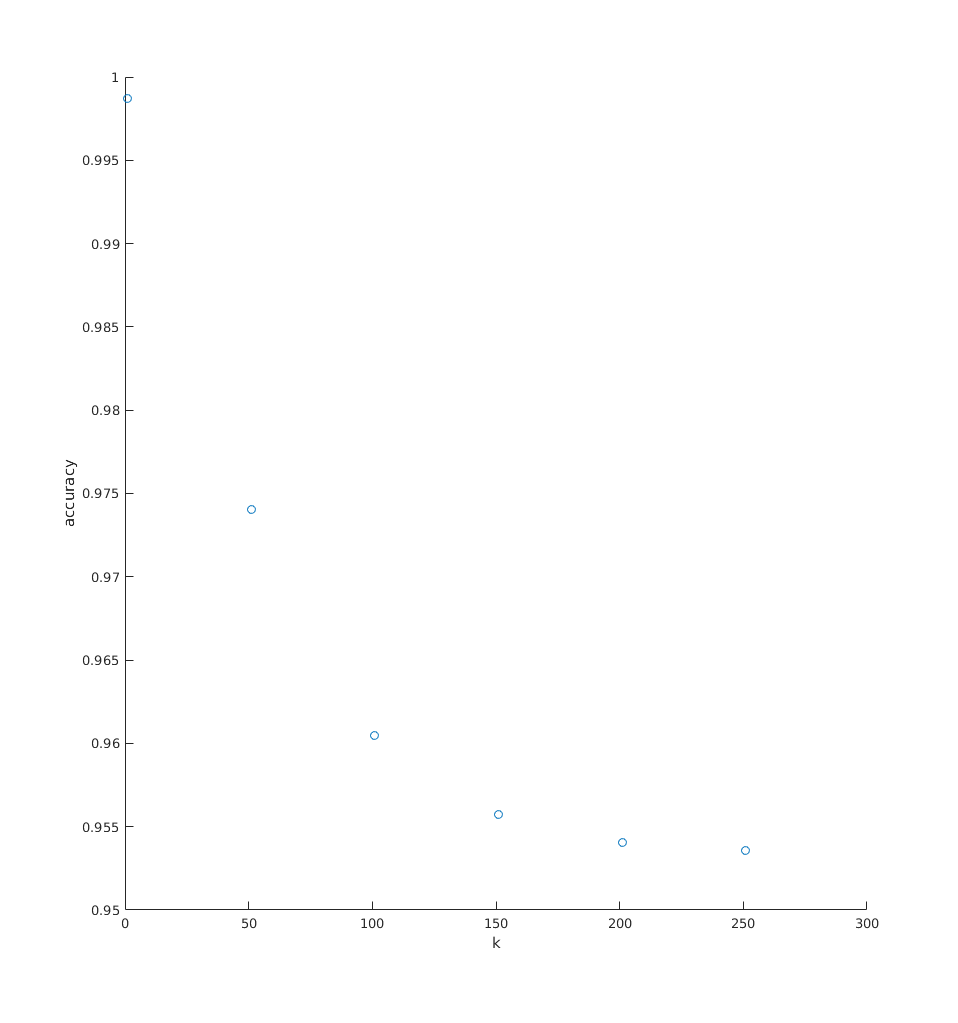
\includegraphics[width=\linewidth]{img/big_k_knn_accu.png}
\caption{Utilizando imágenes grandes}
\end{subfigure}%
\caption{K vs Accuracy con KNN sin PCA}
\end{figure}

En ambos casos obtenemos resultados similares, un accuracy más grande a menor K, siendo K = 1 el valor óptimo, al menos en este caso.
%Dados los resultados, en este caso consideramos que utilizando un valor de K cercano a 10 obtenemos la mejor relación (dentro de nuestro set de tests).\newline
%Por un lado evitamos el problema que ocurre cuando K es demasiado grande y por otro, tomamos una cantidad de imágenes cercanas suficiente como para minimizar el impacto de algún outsider. Aun que cabe destacar que en este caso particular K = 1 tuvo un mejor comportamiento de lo que esperabamos, consideramos que sería arriesgado tomarlo como valor confiable con otros sets de imágenes.

%%%%%%%%%%%%%%%%%%%%%%%%%%%%%%%%%%%%%%%%%%%%%%%%%%%%%%%%%%%%%%%%%%%%%
\begin{figure}[H]
	\centering	
	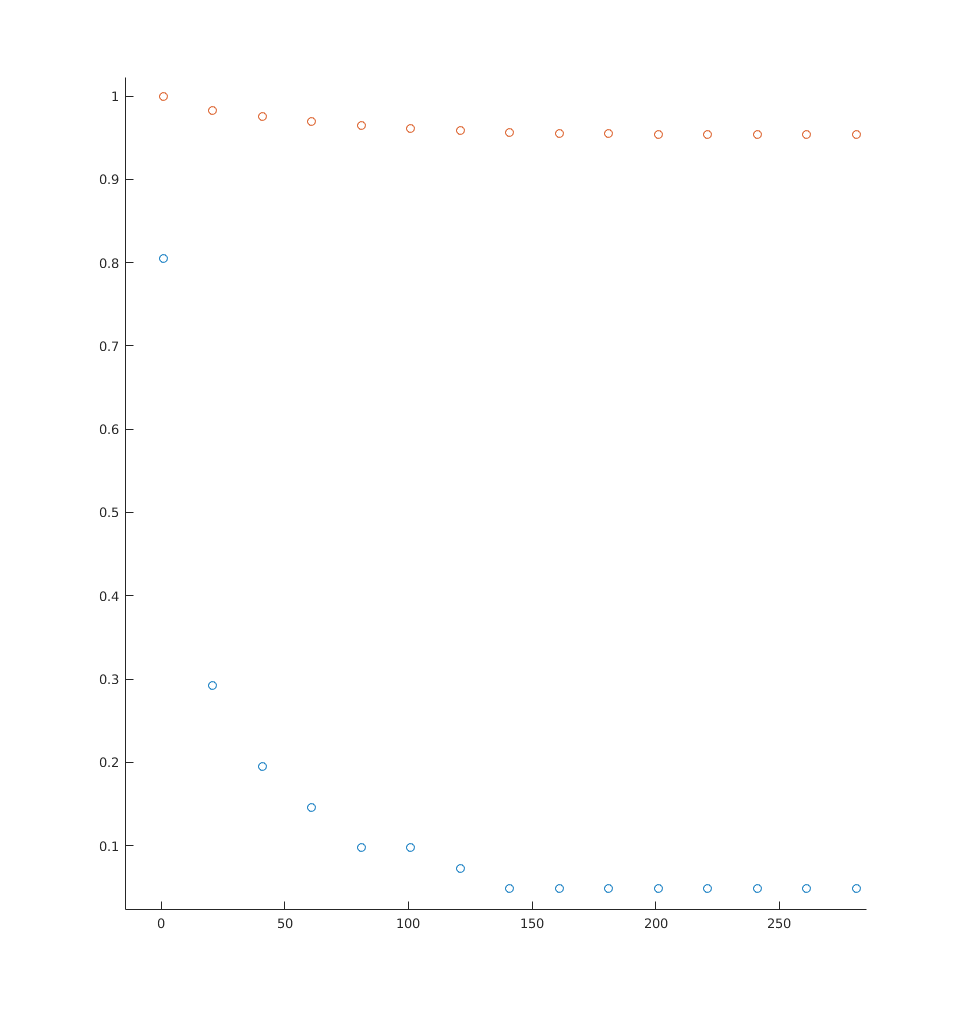
\includegraphics[width=0.8\textwidth]{img/acu_pre.png}
	\caption{Accuracy y precision vs K}
	\label{fig: Accuracy y precision vs K con KNN}
\end{figure}

En este experimento estudiamos cómo la que la cantidad de vecinos cercanos afecta a las métricas Accuracy y Precisión.

Lo que encontramos no fue muy distinto de lo esperado. En la figura anterior vimos la forma en la que Accuracy variaba en función de la cantidad de vecinos cercanos. Pero como explicamos, por ejemplo elegir un K = 250 definitivamente no es una buena elección.Luego en este caso encontramos que Accuracy resulta ser una métrica un tanto engañosa.

Para tener un sistema preciso -valga la redundancia- necesitamos un Valos de (la métrica) Precision relativamente alto. Entonces en función de lo que nos indica el gráfico nuevamente un valor cercano a K = 1 nos parece adecuado.
%%%%%%%%%%%%%%%%%%%%%%%%%%%%%%%%%%%%%%%%%%%%%%%%%%%%%%%%%%%%%%%%%%%%%
\begin{figure}[H]
\begin{subfigure}[h]{0.62\linewidth}
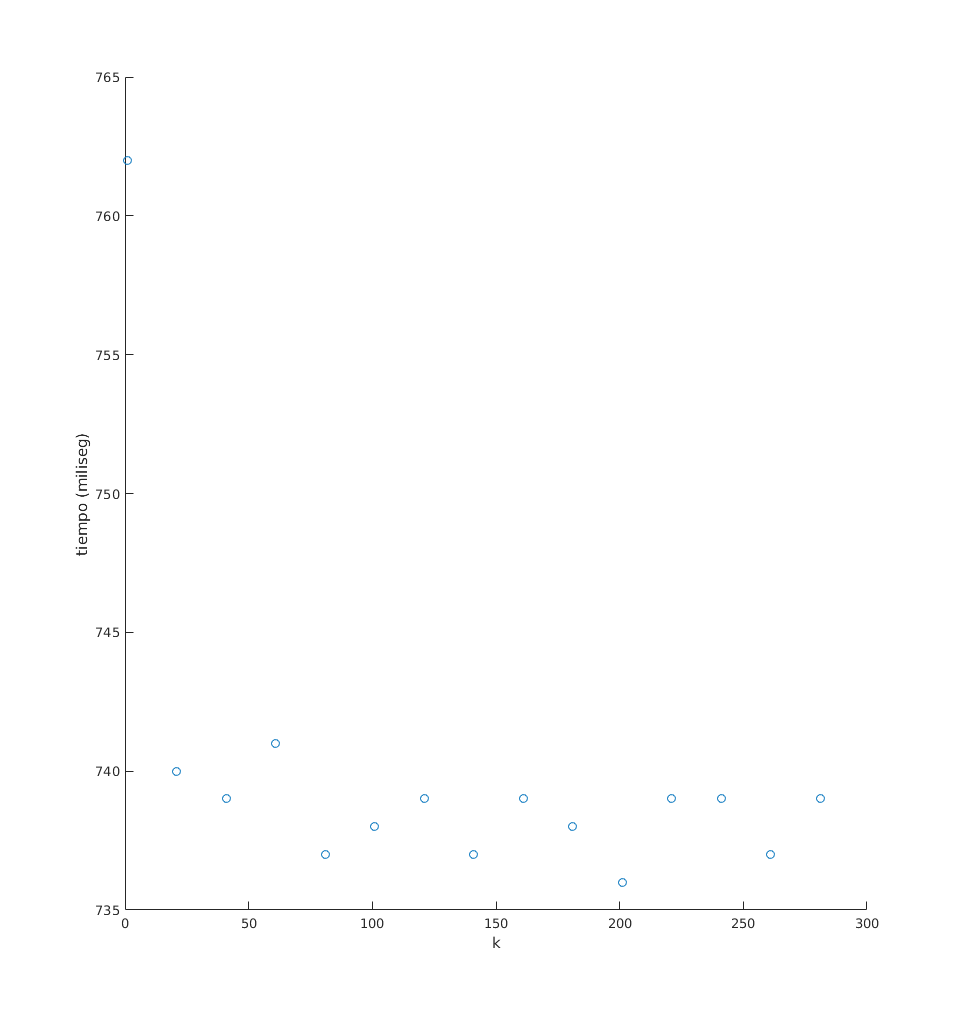
\includegraphics[width=\linewidth]{img/k_knn_tiempo.png}
\caption{Utilizando imágenes reducidas}
\end{subfigure}
\hfill
\begin{subfigure}[h]{0.62\linewidth}
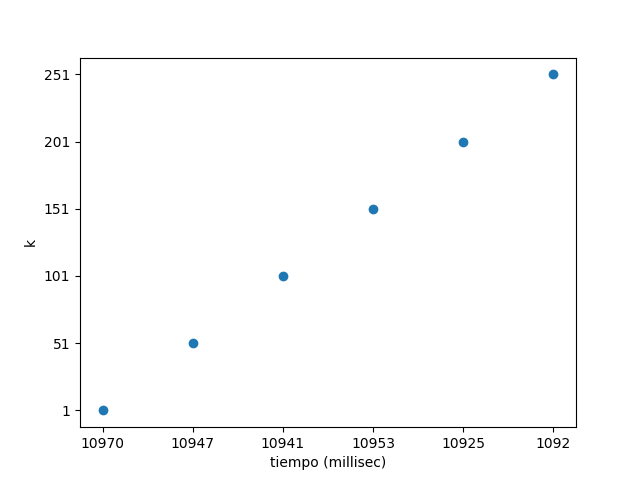
\includegraphics[width=\linewidth]{img/big_k_knn_tiempo.png}
\caption{Utilizando imágenes grandes}
\end{subfigure}%
\caption{K vs tiempo con KNN sin PCA}
\end{figure}


En este caso no logramos identificar ningún patrón evidente. Si bien en el segundo gráfico se observan algúnas diferencias, en realidad representan pequeñas variaciones en el tiempo de ejecución que no consideramos relevantes.
Esto nos parece muy razonable, dado que por la forma de nuestra implementación calculamos la distancia con cada una de las imágenes y elegir un K mayor implica muy pocos cálculos adicionales.
%%%%%%%%%%%%%%%%%%%%%%%%%%%%%%%%%%%%%%%%%%%%%%%%%%%%%%%%%%%%%%%%%%%%%

\begin{figure}[H]
	\centering
	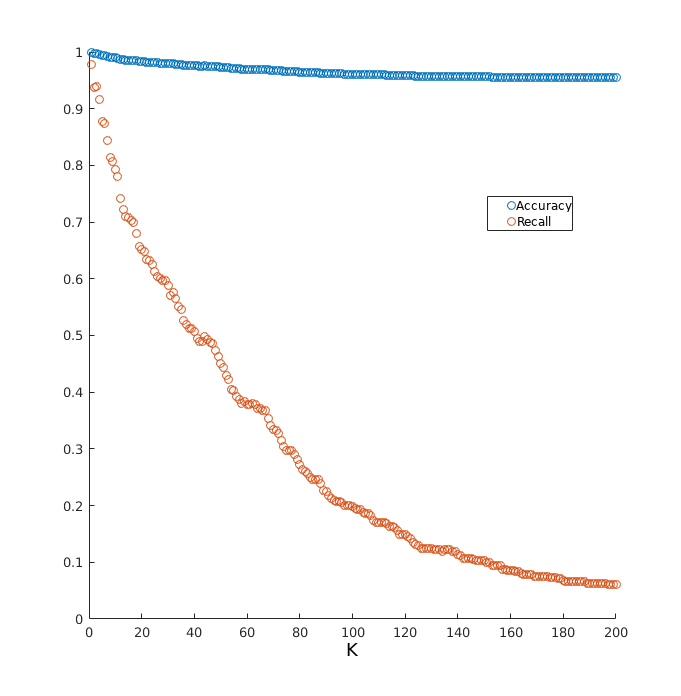
\includegraphics[width=0.8\textwidth]{img/Acc_recall_k_knn.png}
	\caption{Accuracy y Recall vs K (sin PCA)}
	\label{fig: Accuracy y Recall vs K (sin PCA)}
\end{figure}




%%%%%%%%%%%%%%%%%%%%%%%%%%%%%%%%%%%%%%%%%%%%%%%%%%%%%%%%%%%%%%%%%%%%%




\subsubsection*{Conclusiones del test}
Dados los resultados resulta evidente que cuánto más chico el K mejor se comportan nuestras métricas, luego concluímos que K = 1 es el valor óptimo.
Esto tiene sentido, sin embargo si tuvieramos que implementar este problema en la vida real creemos que nos encontraríamos con outlayers que pueden afectar el resultado, ya que con un solo vecino cercano tenemos un sistema poco robusto, por lo que elegiríamos un K un poco más grande, alrededor de 5.






%%%%%%%%%%%%%%%%%%%%%%%%%%%%%%%%%%%%%%%%%%%%%%%%%%%%%%%%%%%%%%%%%%%%%
\subsubsection*{Test con KNN + PCA}
Aquí evaluamos cómo se comporta nuestra implementación con PCA, para eso vamos a repetir los tests anteriores pero esta vez utilizando KNN + PCA.
De acuerdo a lo concluído de los tests anteriores inferimos que utilizar K = 1 o algún valor cercano sería lo mejor. 



%%%%%%%%%%%%%%%%%%%%%%%%%%%%%%%%%%%%%%%%%%%%%%%%%%%%%%%%%%%%%%%%%%%%%
\begin{figure}[H]
	\centering
	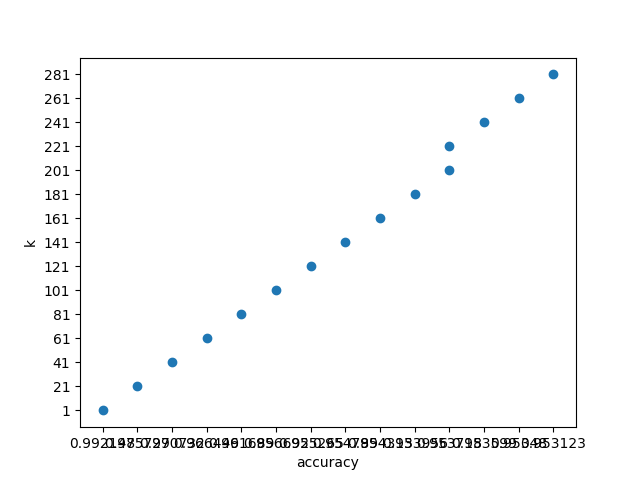
\includegraphics[width=0.8\textwidth]{img/k_pca_accu.png}
	\caption{Accuracy vs K con KNN + PCA}
	\label{fig:K vs Accuracy con KNN + PCA}
\end{figure}

En este caso observamos una estrecha relación entre cuántos vecinos cercanos tomamos y el accuracy.
Nuevamente K = 1 parece ser el valor óptimo.

%%%%%%%%%%%%%%%%%%%%%%%%%%%%%%%%%%%%%%%%%%%%%%%%%%%%%%%%%%%%%%%%%%%%%

\begin{figure}[H]
\begin{subfigure}[h]{0.62\linewidth}
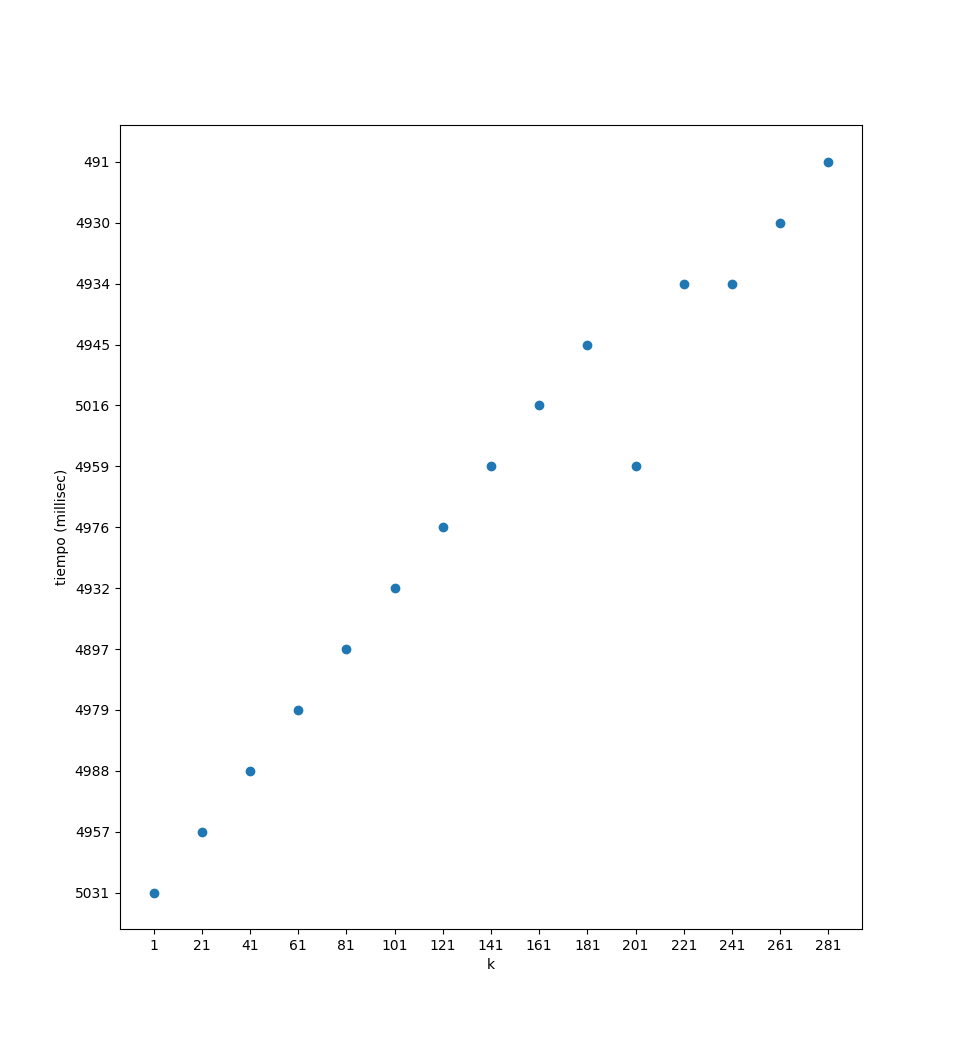
\includegraphics[width=\linewidth]{img/k_pca_tiempo.png}
\caption{Utilizando imágenes reducidas}
\end{subfigure}
\hfill
\begin{subfigure}[h]{0.62\linewidth}
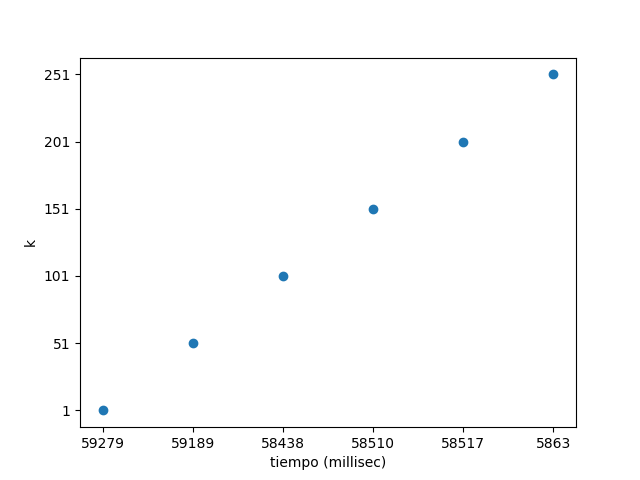
\includegraphics[width=\linewidth]{img/big_k_pca_tiempo.png}
\caption{Utilizando imágenes grandes}
\end{subfigure}%
\caption{K vs tiempo con KNN+PCA}
\end{figure}
Este caso es muy similar al visto sin PCA (Figura 3), no notamos diferencias relevantes.
%Cuidado, tarda un poco más, pero es por el PCA.

%%%%%%%%%%%%%%%%%%%%%%%%%%%%%%%%%%%%%%%%%%%%%%%%%%%%%%%%%%%%%%%%%%%%%

\begin{figure}[H]
\begin{subfigure}[h]{0.62\linewidth}
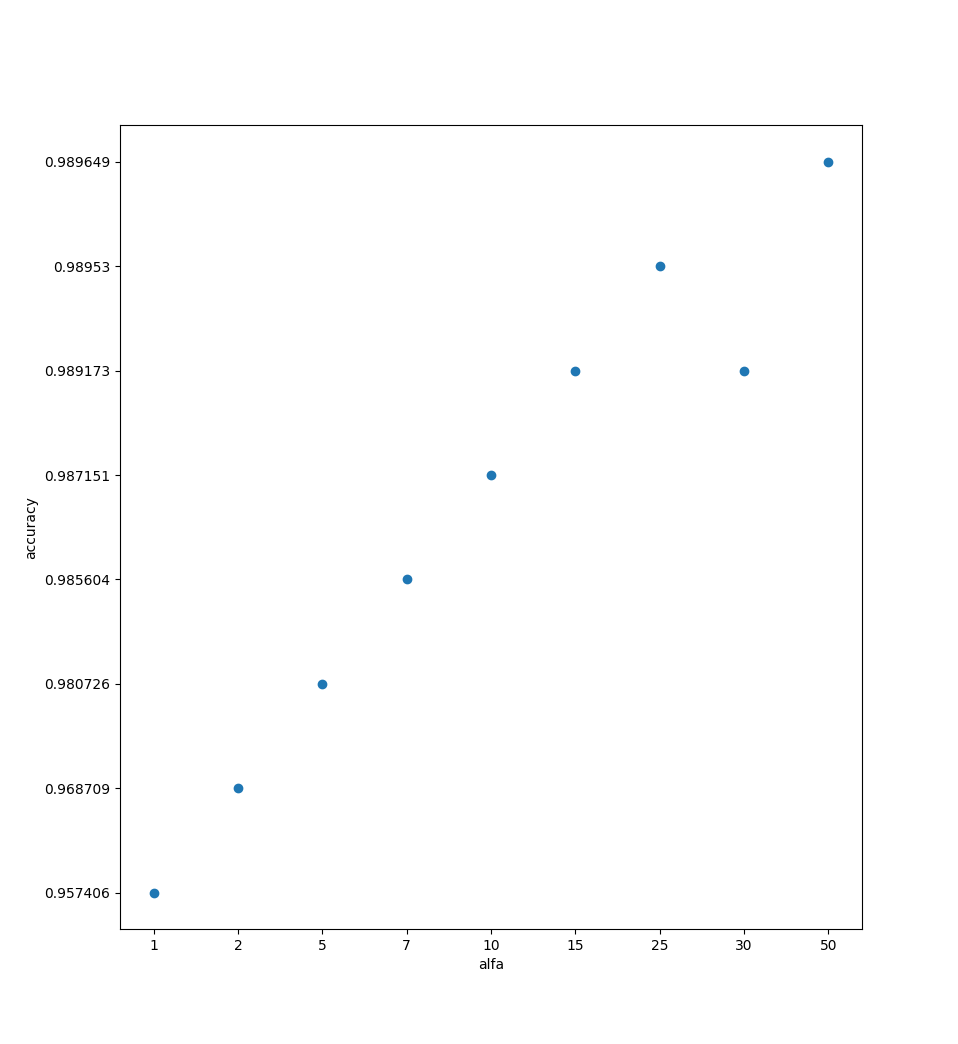
\includegraphics[width=\linewidth]{img/alfa_pca_accu.png}
\caption{Utilizando imágenes reducidas}
\end{subfigure}
\hfill
\begin{subfigure}[h]{0.62\linewidth}
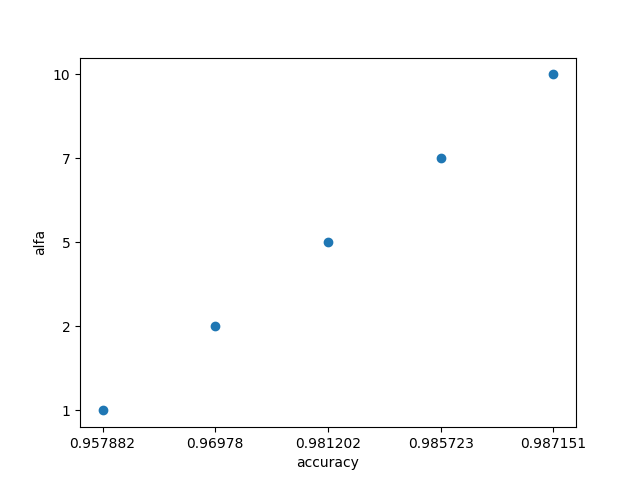
\includegraphics[width=\linewidth]{img/big_alfa_pca_accu.png}
\caption{Utilizando imágenes grandes}
\end{subfigure}%
\caption{Accuracy vs $\alpha$ con KNN+PCA}
\end{figure}

En este caso podemos observar una relación entre las dos variables, a medida que el $\alpha$ aumenta vemos como también lo hace nuestro accuracy.
Como expresamos anteriormente, debido al funcionamiento de PCA esperábamos que a mayor $\alpha$, mejores sean nuestros resultados (todas nuestras métricas en general) y por lo tanto nuestro accuracy también.

Pero a su vez tambien vimos que un $\alpha$ muy elevado  nos elevaría el tiempo de ejecución y a su vez en este gráfico vemos como las diferencias entre accuracy son cada vez menores (por ejemplo entre $\alpha$ = 10 y $\alpha$ = 50).

En base a los resultados obtenidos concluimos que un valor de $\alpha$ cercano a 10 nos daría un buen balance entre relativamente la cantidad de componentes principales y la efectividad (se sacrifica algo de efectividad pero a cambio trabajamos con imágenes mucho más chicas, reduciendo el tiempo de ejecución).

%%%%%%%%%%%%%%%%%%%%%%%%%%%%%%%%%%%%%%%%%%%%%%%%%%%%%%%%%%%%%%%%%%%%%
\begin{figure}[H]
\begin{subfigure}[h]{0.62\linewidth}
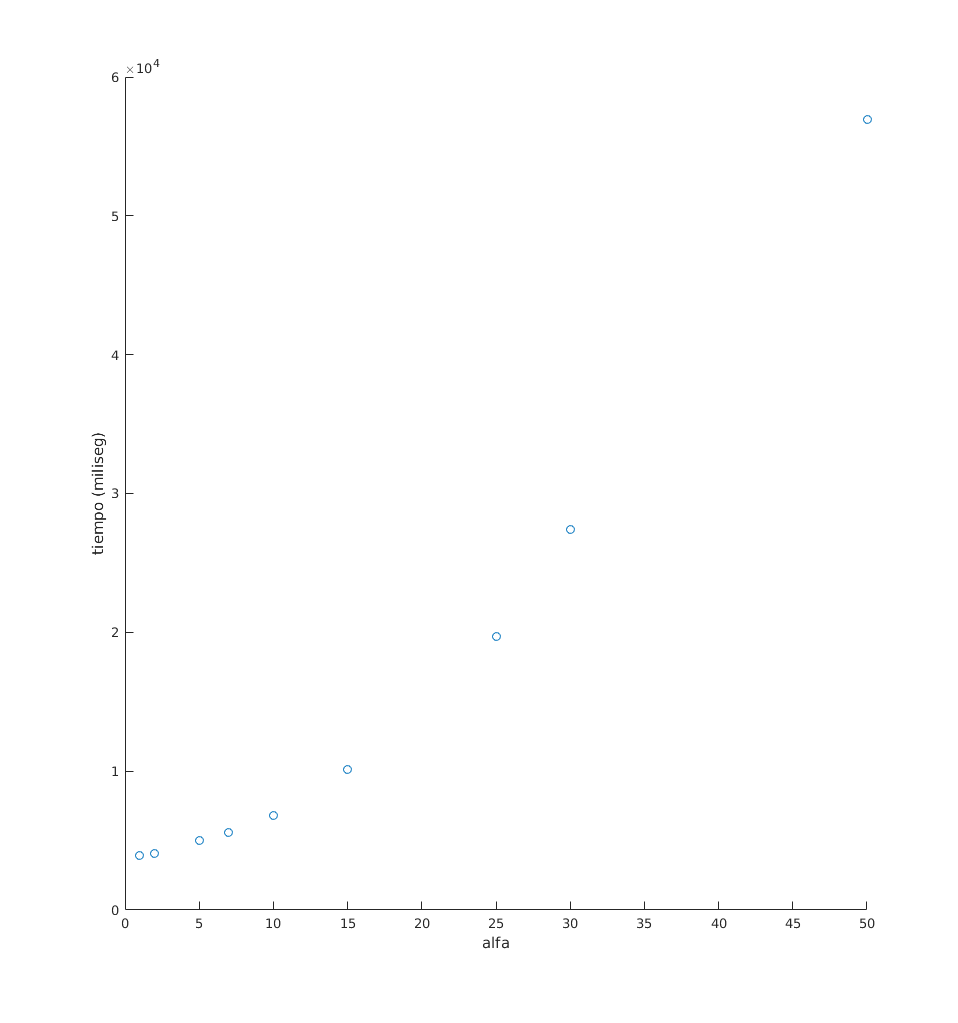
\includegraphics[width=\linewidth]{img/alfa_pca_tiempo.png}
\caption{Utilizando imágenes reducidas}
\end{subfigure}
\hfill
\begin{subfigure}[h]{0.62\linewidth}
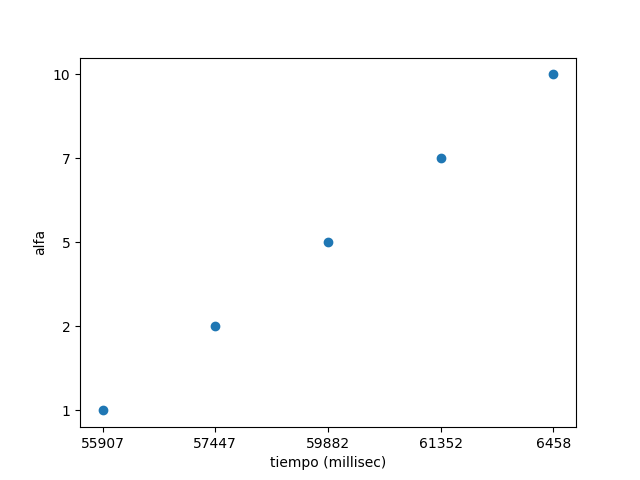
\includegraphics[width=\linewidth]{img/big_alfa_pca_tiempo.png}
\caption{Utilizando imágenes grandes}
\end{subfigure}%
\caption{Tiempo vs $\alpha$ con KNN+PCA}
\end{figure}

Tal como esperabamos vemos que a medida que el $\alpha$ aumenta (es decir, cuantas más componentes principales tengamos), el tiempo de ejecución también lo hace.

Luego, en línea con los resultados de los gráficos anteriores (Accuracy vs $\alpha$) podemos volver a afirmar que un $\alpha$ cercano a 10 sería un buen balance. En este gráfico notamos si tomaramos $\alpha$ = 30, tardaría aproximadamente el triple y no obtendríamos una mejora sustancial en el accuracy.
%%%%%%%%%%%%%%%%%%%%%%%%%%%%%%%%%%%%%%%%%%%%%%%%%%%%%%%%%%%%%%%%%%%%%
\begin{figure}[H]
	\centering
	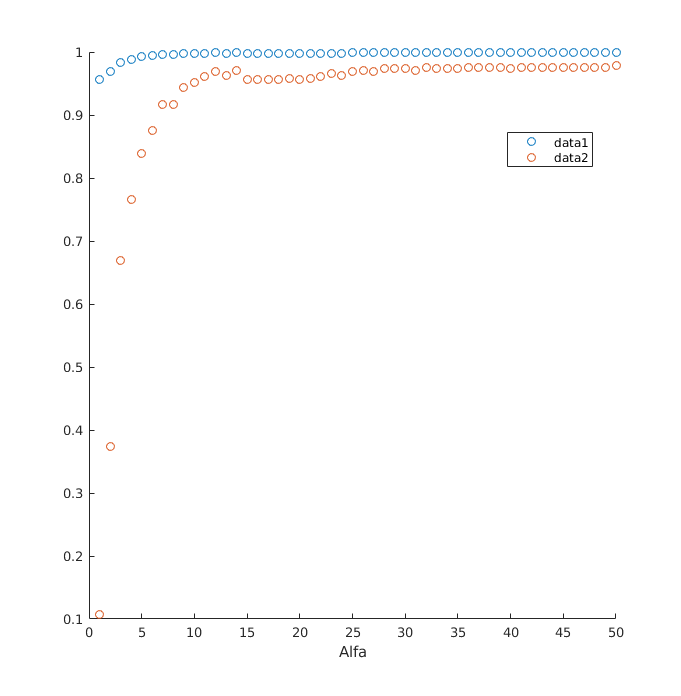
\includegraphics[width=0.8\textwidth]{img/Acc_recall_alfa_pca.png}
	\caption{Accuracy y Recall vs Alfa (con PCA)}
	\label{fig: Accuracy y Recall vs Alfa (con PCA)}
\end{figure}
%%%%%%%%%%%%%%%%%%%%%%%%%%%%%%%%%%%%%%%%%%%%%%%%%%%%%%%%%%%%%%%%%%%%%

\begin{figure}[H]
	\centering
	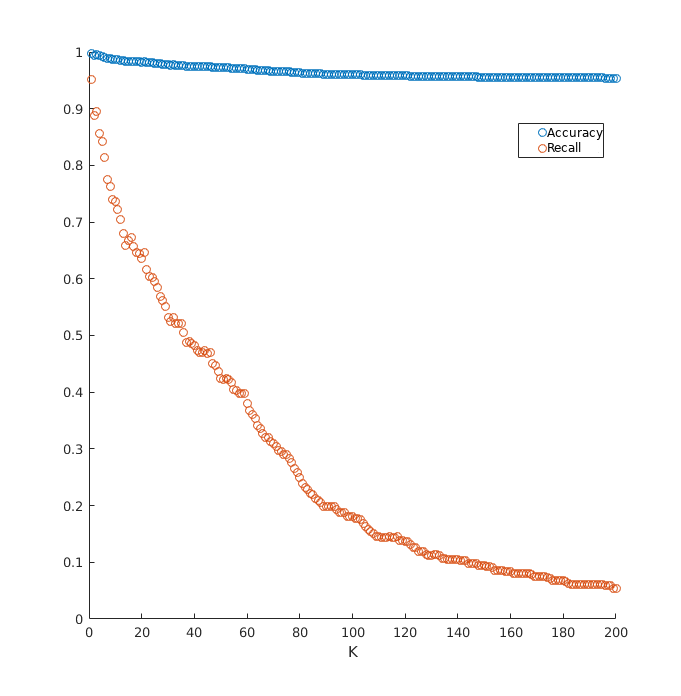
\includegraphics[width=0.8\textwidth]{img/Acc_recall_k_pca.png}
	\caption{Accuracy y Recall vs K (con PCA)}
	\label{fig: Accuracy y Recall vs K (con PCA)}
\end{figure}

%%%%%%%%%%%%%%%%%%%%%%%%%%%%%%%%%%%%%%%%%%%%%%%%%%%%%%%%%%%%%%%%%%%%%

Es llegamos a la conclusión de que utilizando un valor de K cercano a 10 obtenemos la mejor relación (dentro de nuestro set de tests).
Por un lado evitamos el problema que ocurre cuando K es demasiado grande y por otro, tomamos una cantidad de imágenes cercanas suficiente como para minimizar el impacto de algún outsider.


